\documentclass[11pt]{article}
\usepackage{psfig}
\usepackage{framed}
\usepackage{latexsym}
\usepackage{amsfonts,amsmath,amssymb}
\usepackage{graphicx}
\usepackage{caption}
\captionsetup[figure]{labelfont=bf}
\usepackage{hyperref}
\usepackage{enumerate}
%\graphicspath{ {images/} }
\newcommand{\BigO}[1]{\ensuremath{\operatorname{O}\left(#1\right)}}
\interfootnotelinepenalty = 10000
\renewcommand{\thefootnote}{\roman{footnote}}

%\usepackage{amsmath,amssymb,amsthm}
%\theoremstyle{definition}
%\newtheorem{defn}{Definition}[section]

\setlength{\textheight}{8.5in}
\setlength{\textwidth}{6.0in}
\setlength{\headheight}{0in}
\addtolength{\topmargin}{-.5in}
\addtolength{\oddsidemargin}{-.5in}


%--------------
%% preamble.tex
%% this should be included with a command like
%% %--------------
%% preamble.tex
%% this should be included with a command like
%% %--------------
%% preamble.tex
%% this should be included with a command like
%% \input{preamble.tex}
%% \lecture{``lecture number''}{``date''}{``name of professor''}{``name
%%  of student''}

\hbadness=10000
\vbadness=10000

\newcommand{\handout}[5]{
   \renewcommand{\thepage}{\arabic{page}}
   \noindent
   \begin{center}
   \framebox{
      \vbox{
    \hbox to 5.78in { {\bf E2 204: Stochastic Processes and Queuing Theory}
     	 \hfill #1 }
       \vspace{4mm}
       \hbox to 5.78in { {\Large \hfill #4  \hfill} }
       \vspace{2mm}
       \hbox to 5.78in { {\it #2 \hfill #3} }
      }
   }
   \end{center}
   \vspace*{4mm}
}

%\usepackage{amsmath,amssymb,amsthm}
%\theoremstyle{definition}
%\newtheorem{defn}{Definition}[section]

\newcommand{\lecture}[4]{\handout{#1}{Instructor: #2}{Submitted by: #3}{Efficient Collection and Exchange of Information on a Cycle}}

\def\epsilon{\varepsilon}
\def\phi{\varphi}
\def\bool{\{0,1\}}
\def\poly{{\sf poly}}
\def\cross{\times}

\newcommand{\xor}{\oplus}
\newcommand{\Xor}{\bigoplus}
\newcommand{\ceil}[1]{\left\lceil {#1} \right\rceil}
\newcommand{\floor}[1]{\left\lfloor #1 \right\rfloor}
\newcommand{\ignore}[1]{}
\newcommand{\integers}[1]{{\mathbb Z}_{#1}}
\newcommand{\bydef}{\stackrel{\rm def}{=}}
\newcommand{\isequal}{\stackrel{\rm ?}{=}}
\newcommand{\compeq}{\stackrel{\rm c}{\equiv}} % computationally indistinguishable

\newcommand{\qed}{\hspace*{\fill}\rule{7pt}{7pt}}
\newenvironment{proof_sketch}{\noindent{\bf Sketch of Proof} (Informal)\hspace*{1em}}{\qed\medskip}
\newenvironment{proof}{\noindent{\bf Proof}\hspace*{1em}}{\qed\medskip}
\newenvironment{proofof}[1]{\noindent{\bf Proof} of #1:\hspace*{1em}}{\qed\medskip}
%\newenvironment{claim}{\noindent{\bf Claim}\hspace*{1em}\begin{em}}{\end{em}\medskip}
\newcounter{defcounter}
\setcounter{defcounter}{1}
\newenvironment{definition}{\medskip\noindent{\bf Definition }}{\hspace*{\fill}$\diamondsuit$\stepcounter{defcounter}\medskip}
\newtheorem{theorem}{Theorem}
\newtheorem{corollary}[theorem]{Corollary}
\newtheorem{lemma}[theorem]{Lemma}
\newtheorem{claim}[theorem]{Claim}
\newtheorem{fact}[theorem]{Fact}
\newtheorem{conjecture}[theorem]{Conjecture}
\newenvironment{assumption}{\noindent{\bf Assumption}\hspace*{1em}\begin{em}}{\end{em}\medskip}
\newenvironment{remark}{\noindent{\bf Remark}\hspace*{1em}}{\bigskip}

\ignore{
\newcommand{\FOR}{{\bf for}}
\newcommand{\TO}{{\bf to}}
\newcommand{\DO}{{\bf do}}
\newcommand{\WHILE}{{\bf while}}
\newcommand{\AND}{{\bf and}}
\newcommand{\IF}{{\bf if}}
\newcommand{\THEN}{{\bf then}}
\newcommand{\ELSE}{{\bf else}}

%%% You probably will not need to use the commands listed below

\makeatletter
\def\fnum@figure{{\bf Figure \thefigure}}
\def\fnum@table{{\bf Table \thetable}}
\long\def\@mycaption#1[#2]#3{\addcontentsline{\csname
  ext@#1\endcsname}{#1}{\protect\numberline{\csname
  the#1\endcsname}{\ignorespaces #2}}\par
  \begingroup
    \@parboxrestore
    \small
    \@makecaption{\csname fnum@#1\endcsname}{\ignorespaces #3}\par
  \endgroup}
\def\mycaption{\refstepcounter\@captype \@dblarg{\@mycaption\@captype}}
\makeatother

\newcommand{\figcaption}[1]{\mycaption[]{#1}}
\newcommand{\tabcaption}[1]{\mycaption[]{#1}}
\newcommand{\head}[1]{\chapter[Lecture \##1]{}}
\newcommand{\mathify}[1]{\ifmmode{#1}\else\mbox{$#1$}\fi}
\def\half{\frac{1}{2}}

\newcommand{\fig}[4]{
        \begin{figure}
        \setlength{\epsfysize}{#2}
        \vspace{3mm}
        \centerline{\epsfbox{#4}}
        \caption{#3} \label{#1}
        \end{figure}
        }
}

%% \lecture{``lecture number''}{``date''}{``name of professor''}{``name
%%  of student''}

\hbadness=10000
\vbadness=10000

\newcommand{\handout}[5]{
   \renewcommand{\thepage}{\arabic{page}}
   \noindent
   \begin{center}
   \framebox{
      \vbox{
    \hbox to 5.78in { {\bf E2 204: Stochastic Processes and Queuing Theory}
     	 \hfill #1 }
       \vspace{4mm}
       \hbox to 5.78in { {\Large \hfill #4  \hfill} }
       \vspace{2mm}
       \hbox to 5.78in { {\it #2 \hfill #3} }
      }
   }
   \end{center}
   \vspace*{4mm}
}

%\usepackage{amsmath,amssymb,amsthm}
%\theoremstyle{definition}
%\newtheorem{defn}{Definition}[section]

\newcommand{\lecture}[4]{\handout{#1}{Instructor: #2}{Submitted by: #3}{Efficient Collection and Exchange of Information on a Cycle}}

\def\epsilon{\varepsilon}
\def\phi{\varphi}
\def\bool{\{0,1\}}
\def\poly{{\sf poly}}
\def\cross{\times}

\newcommand{\xor}{\oplus}
\newcommand{\Xor}{\bigoplus}
\newcommand{\ceil}[1]{\left\lceil {#1} \right\rceil}
\newcommand{\floor}[1]{\left\lfloor #1 \right\rfloor}
\newcommand{\ignore}[1]{}
\newcommand{\integers}[1]{{\mathbb Z}_{#1}}
\newcommand{\bydef}{\stackrel{\rm def}{=}}
\newcommand{\isequal}{\stackrel{\rm ?}{=}}
\newcommand{\compeq}{\stackrel{\rm c}{\equiv}} % computationally indistinguishable

\newcommand{\qed}{\hspace*{\fill}\rule{7pt}{7pt}}
\newenvironment{proof_sketch}{\noindent{\bf Sketch of Proof} (Informal)\hspace*{1em}}{\qed\medskip}
\newenvironment{proof}{\noindent{\bf Proof}\hspace*{1em}}{\qed\medskip}
\newenvironment{proofof}[1]{\noindent{\bf Proof} of #1:\hspace*{1em}}{\qed\medskip}
%\newenvironment{claim}{\noindent{\bf Claim}\hspace*{1em}\begin{em}}{\end{em}\medskip}
\newcounter{defcounter}
\setcounter{defcounter}{1}
\newenvironment{definition}{\medskip\noindent{\bf Definition }}{\hspace*{\fill}$\diamondsuit$\stepcounter{defcounter}\medskip}
\newtheorem{theorem}{Theorem}
\newtheorem{corollary}[theorem]{Corollary}
\newtheorem{lemma}[theorem]{Lemma}
\newtheorem{claim}[theorem]{Claim}
\newtheorem{fact}[theorem]{Fact}
\newtheorem{conjecture}[theorem]{Conjecture}
\newenvironment{assumption}{\noindent{\bf Assumption}\hspace*{1em}\begin{em}}{\end{em}\medskip}
\newenvironment{remark}{\noindent{\bf Remark}\hspace*{1em}}{\bigskip}

\ignore{
\newcommand{\FOR}{{\bf for}}
\newcommand{\TO}{{\bf to}}
\newcommand{\DO}{{\bf do}}
\newcommand{\WHILE}{{\bf while}}
\newcommand{\AND}{{\bf and}}
\newcommand{\IF}{{\bf if}}
\newcommand{\THEN}{{\bf then}}
\newcommand{\ELSE}{{\bf else}}

%%% You probably will not need to use the commands listed below

\makeatletter
\def\fnum@figure{{\bf Figure \thefigure}}
\def\fnum@table{{\bf Table \thetable}}
\long\def\@mycaption#1[#2]#3{\addcontentsline{\csname
  ext@#1\endcsname}{#1}{\protect\numberline{\csname
  the#1\endcsname}{\ignorespaces #2}}\par
  \begingroup
    \@parboxrestore
    \small
    \@makecaption{\csname fnum@#1\endcsname}{\ignorespaces #3}\par
  \endgroup}
\def\mycaption{\refstepcounter\@captype \@dblarg{\@mycaption\@captype}}
\makeatother

\newcommand{\figcaption}[1]{\mycaption[]{#1}}
\newcommand{\tabcaption}[1]{\mycaption[]{#1}}
\newcommand{\head}[1]{\chapter[Lecture \##1]{}}
\newcommand{\mathify}[1]{\ifmmode{#1}\else\mbox{$#1$}\fi}
\def\half{\frac{1}{2}}

\newcommand{\fig}[4]{
        \begin{figure}
        \setlength{\epsfysize}{#2}
        \vspace{3mm}
        \centerline{\epsfbox{#4}}
        \caption{#3} \label{#1}
        \end{figure}
        }
}

%% \lecture{``lecture number''}{``date''}{``name of professor''}{``name
%%  of student''}

\hbadness=10000
\vbadness=10000

\newcommand{\handout}[5]{
   \renewcommand{\thepage}{\arabic{page}}
   \noindent
   \begin{center}
   \framebox{
      \vbox{
    \hbox to 5.78in { {\bf E2 204: Stochastic Processes and Queuing Theory}
     	 \hfill #1 }
       \vspace{4mm}
       \hbox to 5.78in { {\Large \hfill #4  \hfill} }
       \vspace{2mm}
       \hbox to 5.78in { {\it #2 \hfill #3} }
      }
   }
   \end{center}
   \vspace*{4mm}
}

%\usepackage{amsmath,amssymb,amsthm}
%\theoremstyle{definition}
%\newtheorem{defn}{Definition}[section]

\newcommand{\lecture}[4]{\handout{#1}{Instructor: #2}{Submitted by: #3}{Efficient Collection and Exchange of Information on a Cycle}}

\def\epsilon{\varepsilon}
\def\phi{\varphi}
\def\bool{\{0,1\}}
\def\poly{{\sf poly}}
\def\cross{\times}

\newcommand{\xor}{\oplus}
\newcommand{\Xor}{\bigoplus}
\newcommand{\ceil}[1]{\left\lceil {#1} \right\rceil}
\newcommand{\floor}[1]{\left\lfloor #1 \right\rfloor}
\newcommand{\ignore}[1]{}
\newcommand{\integers}[1]{{\mathbb Z}_{#1}}
\newcommand{\bydef}{\stackrel{\rm def}{=}}
\newcommand{\isequal}{\stackrel{\rm ?}{=}}
\newcommand{\compeq}{\stackrel{\rm c}{\equiv}} % computationally indistinguishable

\newcommand{\qed}{\hspace*{\fill}\rule{7pt}{7pt}}
\newenvironment{proof_sketch}{\noindent{\bf Sketch of Proof} (Informal)\hspace*{1em}}{\qed\medskip}
\newenvironment{proof}{\noindent{\bf Proof}\hspace*{1em}}{\qed\medskip}
\newenvironment{proofof}[1]{\noindent{\bf Proof} of #1:\hspace*{1em}}{\qed\medskip}
%\newenvironment{claim}{\noindent{\bf Claim}\hspace*{1em}\begin{em}}{\end{em}\medskip}
\newcounter{defcounter}
\setcounter{defcounter}{1}
\newenvironment{definition}{\medskip\noindent{\bf Definition }}{\hspace*{\fill}$\diamondsuit$\stepcounter{defcounter}\medskip}
\newtheorem{theorem}{Theorem}
\newtheorem{corollary}[theorem]{Corollary}
\newtheorem{lemma}[theorem]{Lemma}
\newtheorem{claim}[theorem]{Claim}
\newtheorem{fact}[theorem]{Fact}
\newtheorem{conjecture}[theorem]{Conjecture}
\newenvironment{assumption}{\noindent{\bf Assumption}\hspace*{1em}\begin{em}}{\end{em}\medskip}
\newenvironment{remark}{\noindent{\bf Remark}\hspace*{1em}}{\bigskip}

\ignore{
\newcommand{\FOR}{{\bf for}}
\newcommand{\TO}{{\bf to}}
\newcommand{\DO}{{\bf do}}
\newcommand{\WHILE}{{\bf while}}
\newcommand{\AND}{{\bf and}}
\newcommand{\IF}{{\bf if}}
\newcommand{\THEN}{{\bf then}}
\newcommand{\ELSE}{{\bf else}}

%%% You probably will not need to use the commands listed below

\makeatletter
\def\fnum@figure{{\bf Figure \thefigure}}
\def\fnum@table{{\bf Table \thetable}}
\long\def\@mycaption#1[#2]#3{\addcontentsline{\csname
  ext@#1\endcsname}{#1}{\protect\numberline{\csname
  the#1\endcsname}{\ignorespaces #2}}\par
  \begingroup
    \@parboxrestore
    \small
    \@makecaption{\csname fnum@#1\endcsname}{\ignorespaces #3}\par
  \endgroup}
\def\mycaption{\refstepcounter\@captype \@dblarg{\@mycaption\@captype}}
\makeatother

\newcommand{\figcaption}[1]{\mycaption[]{#1}}
\newcommand{\tabcaption}[1]{\mycaption[]{#1}}
\newcommand{\head}[1]{\chapter[Lecture \##1]{}}
\newcommand{\mathify}[1]{\ifmmode{#1}\else\mbox{$#1$}\fi}
\def\half{\frac{1}{2}}

\newcommand{\fig}[4]{
        \begin{figure}
        \setlength{\epsfysize}{#2}
        \vspace{3mm}
        \centerline{\epsfbox{#4}}
        \caption{#3} \label{#1}
        \end{figure}
        }
}


\newcommand{\problembreak}{\hfill $\blacksquare$}
%\newcommand{\X}{\mathsf{X}}
%\newcommand{\Y}{\mathsf{Y}}
%\newcommand{\U}{\mathsf{U}}
%\newcommand{\V}{\mathsf{V}}
%\newcommand{\W}{\mathsf{W}}
%\newcommand{\S}{\mathsf{S}}
%\newcommand{\T}{\mathsf{T}}

\begin{document}
	
	\lecture{29th April 2017}{Parimal Parag}{Prateek Kumar Vishwakarma}
	
	
	\section{Introduction}
	Suppose there are a certain number of nodes that lie on a circle and a few number of particles traverse through them. While traversal, the particles collect and carry information about the nodes they pass through, and exchange the information they carry with other particles whenever they meet, given that they can only meet at the nodes.\\
	The answer that we are looking for, is to find out in what way the particles should move, so that each particle has the latest possible information about each node.\\[1mm]
	We will work assuming that there are $\alpha$ number of nodes and 2 particles that traverse independently.\\[1mm]
	We will only focus on making comparisons between 3 cases.
	\begin{figure}[h!]
		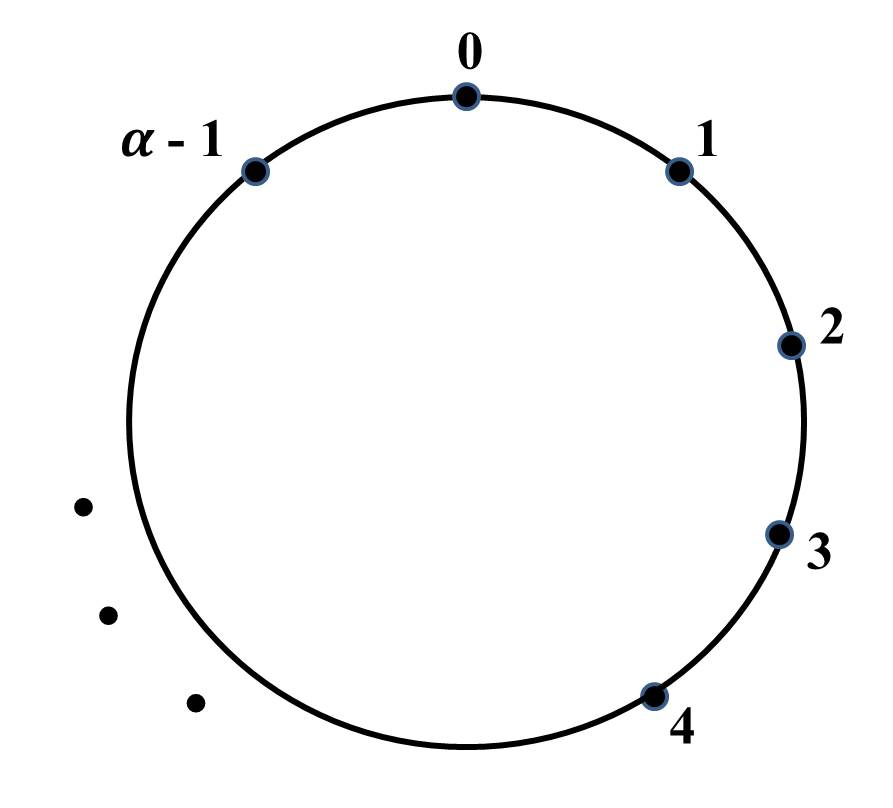
\includegraphics[width=0.40 \columnwidth]{pic1}
		\centering
	\end{figure}
	\section{Definitions and Notations}
	\begin{itemize}
		\item  $X_i$, $Y_i$, $X$, $Y$, $S_n$, $T_n$, $U_n$, $V_n$, $W_n$ will denote real valued random variables.
		\item  $X_i \sim X$ be independent($E[|X|]<\infty$).
		\item $Y_i \sim Y$ be independent ($E[|Y|]<\infty$).
		\item Each $X_i$ and $Y_j$ are independent.
		\item $S_n := \sum_{i=1}^{n} X_i$; $T_n := \sum_{i=1}^{n} Y_i$.
		\item Then $S_n, T_n$ and $S_n - T_n$ are random walks on the line.
		\item $U_n := S_n \; mod \; \alpha$.
		\item  $V_n := T_n \; mod \; \alpha$.
		\item $W_n := (S_n - T_n )\; mod \; \alpha$.
		\item Then $U_n, V_n$ and $W_n$ are random walks on the circle.
	\end{itemize}
	The motion of Particle $1$ is governed by $U_n$ and that of Particle $2$ is governed by $V_n$.
	\section{Considering Different Cases}
	\subsection{Symmetric Case with $E[X_i] = E[Y_i] = 0$}\label{sym}
	$$X := \begin{cases}
	1 &\text{ w.p. } 1/4\\
	-1 &\text{ w.p. } 1/4\\
	0 &\text{ w.p. } 1/2
	\end{cases}$$
	\noindent Let $Y = X$. \\[2mm]
	In this case, $U_n$ and $V_n$ are random walks that move in either direction with probability $1/4$ and stay put with probability $1/2$.\\
	Then, 
	$$E[X_i] = 0 = E[Y_i] \; \implies \; \frac{S_n - T_n}{n} \to E[X_i - Y_i] = 0 \text{ w.p. } 1$$
	$$\implies \; S_n - T_n \sim o(n)$$
	Thus, in this case, we can say that the rate at which $S_n - T_n$ tends to $\pm \infty$ is much less than $n$.
	\subsection{Asymmetric Case with $E[X_i] = E[Y_i] < 0$}\label{asym1}
	$$X := \begin{cases}
	1 &\text{ w.p. } p\\
	-1 &\text{ w.p. } 1/2 - p\\
	0 &\text{ w.p. } 1/2
	\end{cases}$$
	\noindent where $0< p < 1/4$. \\
	Let $Y = X$. \\[2mm]
	Now as $E[X_i] = E[Y_i] < 0 \; \implies S_n \to -\infty$ and $T_n \to -\infty$ as $n \to \infty$.\\
	Intuitively, we can say that Particle $1$ and Particle $2$ will eventually look like moving together in the counterclockwise direction on the circle. \\
	Now, if we try to investigate whether or not the random walk $S_n - T_n$ tends to $\pm \infty$, we can only be sure of one thing that 
	$$S_n - T_n \sim o(n)$$
	This is because $E[X_i - Y_i] = 0$
	$$\implies \frac{S_n - T_n}{n} \to 0 \text{ as } n \to \infty \text{ w.p. } 1$$
	$$\implies S_n - T_n \sim o(n)$$
	So, the rate at which $S_n - T_n$ tends to $+\infty$ is slower than $n$.
	\subsection{Asymmetric Case with $E[X_i] = -E[Y_i]$}\label{asym2}
	$$X := \begin{cases}
	1 &\text{ w.p. } p\\
	-1 &\text{ w.p. } 1/2 - p\\
	0 &\text{ w.p. } 1/2
	\end{cases}$$
	where $0< p < 1/4$.\\
	Let $Y = -X$.\\[2mm]
	As
	$$E[X_i] =p - \frac{1}{2} + p = 2p - \frac{1}{2}< 0 \text{ , and } \frac{S_n}{n} \to E[X_i] \text{ as } n \to \infty \text{ w.p. } 1$$
	therefore, 
	$$S_n \to -\infty \text{ as } n \to \infty$$
	Similarly, 
	$$T_n \to +\infty \text{ as } n \to \infty$$
	So intuitively, we can say that, eventually, Particle $1$ will look like it is moving in counterclockwise direction and Particle $2$ will look like it is moving in the clockwise direction, on the circle.\\
	Now, if we take a look at the random walk $S_n - T_n$, then we can observe that, as $E[X_i - Y_i] < 0$, therefore $S_n -T_n \to -\infty$ w.p. $1$.\\
	This implies that the random walk $S_n - T_n$ will keep hitting multiples of $\alpha$. In other words, $W_n = 0$ for infinitely many $n \in \mathbb{N}$.\\
	Hence, the two particles will keep meeting each other and hence, keep exchanging information they have.
	
	\subsection{Comparison between the three cases}
	\begin{itemize}
		\item In Case \ref{asym2}, Particle $1$ and Particle $2$ eventually start moving in opposite direction, retrieving the information from the nodes more uniformly than in Case \ref{asym1}, in which, Particle $1$ and Particle $2$ eventually start moving in the same direction.
		\item Since in Case \ref{asym2}, Particle $1$ and Particle $2$ look like they are moving in opposite directions, the tendency of particles to meet and efficiently exchange their information in this case is more probable than that in Case \ref{asym1}. This is because, in Case \ref{asym1}, they look like they are moving in the same direction.
		\item Now, Case \ref{sym} and Case \ref{asym1} are not very different from each other. One difference that we emphasize is that the random walk in Case \ref{sym} has more entropy than that in Case \ref{asym1}, which results in particles moving more randomly in Case \ref{sym}. Because of this, the information carried by the particles in Case \ref{sym} is safer\footnote{We can talk about safety if there is a Particle $3$ that, instead of sharing the information, destroys it.} than in Case \ref{asym1}.
	\end{itemize}
	
	\section{Further Questions that we wish to Answer}
	\begin{itemize}
		\item Obviously, we have to formalize the arguments above rigorously.
		\item To find the optimal probability of staying put at a state such that the nodes can be visited by the two particles and can be exchanged frequently (in the cases we considered, that probability  is $1/2$).
		\item Try and generalize the above theory for more than two particles.
		\item To find optimal number of particles (depending on $\alpha$) needed to cover a cycle with $\alpha$ nodes such that, the expenditure\footnote{Suppose deploying each particle costs some money} is minimized and the number of visits to each node is maximized. Further, the particles should meet each other (so that data is exchanged) as frequently as possible. 
		\item Suppose there is another particle, Particle $3$, in addition to Particle $1$ and Particle $2$. Particle $3$ destroys all information carried by another particle with which it collides. So, in order to save the information, the two particles should do their random walks depending on the random walk of Particle $3$. How should they move now, so that they collide with Particle $3$, as less as possible, and yet can perform their jobs successfully?
	\end{itemize}
	
\section*{Acknowledgement}	
I would like to thank Prof. Parimal Parag for introducing this nice problem to me and for his support in all the discussions. 

\begin{thebibliography}{9}
	\bibitem{SMR} 
	Sheldon M. Ross
	\textit{Stochastic Processes}.
	\bibitem{ANS}
	A.N. Shiryaev
	\textit{Probability}.
	\bibitem{net}
	en.wikipedia.org	
\end{thebibliography}
	
\end{document}